% HMC Math dept HW template example
% v0.04 by Eric J. Malm, 10 Mar 2005
\documentclass[12pt,letterpaper,boxed]{hmcpset}

% set 1-inch margins in the document
\usepackage[margin=1in]{geometry}
\usepackage{alltt}
\usepackage{amsfonts}
\usepackage{amsmath}
\usepackage{amssymb}
\usepackage{amsthm}
\usepackage{booktabs}
\usepackage{caption}
\usepackage{fancyhdr}
\usepackage{graphicx}
\usepackage{mathdots}
\usepackage{mathtools}
\usepackage{microtype}
\usepackage{multirow}
\usepackage{pdflscape}
\usepackage{pgfplots}
\usepackage{siunitx}
\usepackage{slashed}
\usepackage{tabularx}
\usepackage{tikz}
\usepackage{tkz-euclide}
\usepackage[normalem]{ulem}
\usepackage[all]{xy}
\usepackage{imakeidx}
\usepackage{enumerate}
\usepackage{physics}

% include this if you want to import graphics files with /includegraphics
\usepackage{graphicx}

\renewcommand{\tt}{t^{(i)}}
\newcommand{\ww}{w^{(i)}}
\renewcommand{\ss}{\sigma^{(i)}}
\newcommand{\ind}[1]{\mathbb{I}\{#1\}}
\DeclareMathOperator*{\argmax}{argmax}
\DeclareMathOperator*{\argmin}{argmin}
\newcommand{\thetamap}{\theta_{\mathrm{MAP}}}
\renewcommand{\diag}{\mathrm{diag}}
\newcommand{\DKL}[2]{D_{\mathrm{KL}}(#1 \parallel #2)}
\newcommand{\lunsup}{\ell_{\mathrm{unsup}}}
\newcommand{\lsup}{\ell_{\mathrm{sup}}}
\newcommand{\lsemi}{\ell_{\mathrm{semi-sup}}}
\newcommand{\tht}{\theta^{(t)}}
\newcommand{\thtt}{\theta^{(t+1)}}
\newcommand{\summ}{\sum_{i=1}^m}
\newcommand{\sumtm}{\sum_{i=1}^{\tilde m}}
\newcommand{\sumsa}{\sum_{(s,a)}}

% info for header block in upper right hand corner
\name{Runqiu Ye}
\class{Stanford CS229}
\assignment{Problem Set \#4}
\duedate{08/07/2024}

\linespread{1.15}
\begin{document}

\problemlist{Problem Set \#3: EM, Deep Learning, \& Reinforcement Learning}

\begin{problem}[Problem 1]
\textbf{Neural Networks: MNIST image classification}

Implement a simple convolutional neural network to classify grayscale images of handwritten digits from the MNIST dataset. The starter code splits the set of 60000 training images and labels into a sets of 59600 examples as the training set and 400 examples for the dev set.

To start, implement convolutional neural network and cross entropy loss, and train it with the provided dataset. The architecture is as follows:
\begin{enumerate}[(a)]
  \item The first layer is a convolutional layer with 2 output channels with a convolution size of 4 by 4.
  \item The second layer is a max pooling layer of stride and width 5 by 5.
  \item The third layer is a ReLU activation layer.
  \item After the four layer, the data is flattened into a single dimension.
  \item The fifth layer is a single linear layer with output size 10 (the number of classes).
  \item The sixth layer is a softmax layer that computes the probabilities for each classes.
  \item Finally, we use a cross entropy loss as our loss function.
\end{enumerate}

The cross entropy loss is
\[
CE(y, \hat y) = - \sum_{k=1}^K y_k \log \hat{y}_k,
\]
where $\hat y \in \R^K$ is the vector of softmax outputs from the model for the training example $x$, and $y \in \R^K$ is the ground-truth vector for the training example $X$ such that $y = [0, \dots, 0, 1, 0, \dots, 0]^T$ contains a single 1 at the position of the correct classes.

We also use mini-batch gradient descent with a batch size of 16. Normally we would iterate over the data multiple times with multiple epochs, but for this assignment we only do 400 batches to save time.
\end{problem}

\begin{solution}
\begin{enumerate}[(a)]
  \item Implement functions within \verb|p01_nn.py|.
  \item Implement a function that computes the full backward pass. See training curve in \verb|src/output/train.png|
\end{enumerate}
\end{solution}

% \newpage
\begin{problem}[Problem 2]
  \textbf{Off Policy Evaluatino And Causal Inference}

  Need methods for evaluating policies without actually implementing them. This task is off-policy evaluation or causal inference.

  For this problem, consider MDPs with a single timestep. Consider universe of states $S$, actions $A$, a reward function $R(s, a)$ where $s$ is a state and $a$ is an action. We often only have a subset of $a$ in our dataset. For eaxmple, each state $s$ could represent a patient, each action $a$ could represent which drug we prescribe to that patient and $R(s, a)$ be their lifespan after prescribing that drug.

  A policy is defined as $\pi_i (s, a) = p(a \mid s, \pi_i)$ We are given observational dataset of $(s, a, R(s, a))$ tuples. Let $p(s)$ be the density for the distribution of the state $s$ values wihin the dataset. Let $\pi_0 (s, a) = p(a \mid s)$ within our observational data. $\pi_0$ corresponds to the baseline policy in observational data. Also given target policy $\pi_1 (s,a)$ which gives the conditional probability $p(a \mid s)$ in our optimal policy. Our goal is to computer expected value of $R(s,a)$ in the same population as our observatinoal data, but with a policy of $\pi_1$ instead of $\pi_0$. In other words, we are trying to compute
  \[
  \E_{\substack{s \sim p(s) \\ a \sim \pi_1(s,a)}} [R(s, a)] = \sum_{(s,a)} R(s,a) p(s,a) = \sum_{(s,a)} R(s,a) p(s) p(a \mid s) = \sum_{(s,a)} R(s,a) p(s) \pi_1 (s,a).
  \]

  \textbf{Simplifying Assumptions: } We will assume that each action has a non-zero probability in the observed policy $\pi_0 (s, a)$. In other words, for all actions $a$ and states $s$, $\pi_0 (s,a) > 0$.

  \textbf{Regression:} The simplest possible estimator is to directly use our learned MDP parameters to estimate our goal. This is called regression estimator. While training our MDP, we learn an estimator $\hat R(s,a)$ that estimates $R(s,a)$. We can now directly estimate
  \[
  \E_{\substack{s \sim p(s) \\ a \sim \pi_1(s,a)}} [R(s, a)]
  \]
  with 
  \[
    \E_{\substack{s \sim p(s) \\ a \sim \pi_1(s,a)}} [\hat R(s, a)].
  \]
  If $\hat R(s,a) = R(s,a)$, then this estimator is trivially correct. We will now consider alternative approaches and explore why you might use one estimator over another.
\end{problem}

\begin{solution}
  \begin{enumerate}[(a)]
    \item \textbf{Importance Sampling:} Let $\hat \pi_0$ be an estimate of the true $\pi_0$. The \emph{importance sampling estimator} uses that $\hat \pi_0$ and has the form 
    \[
    \E_{\substack{s \sim p(s) \\ a \sim \pi_0 (s,a)}} \qty[\frac{\pi_1(s,a)}{\hat \pi_0 (s,a)} R(s,a)].
    \]
    We now show that if $\hat \pi_0 = \pi_0$, then the importance sampling estimator is equal to 
    \[
    \E_{\substack{s \sim p(s) \\ a \sim \pi_1(s,a)}} [R(s,a)].
    \]
    
    \begin{proof}
      If $\hat \pi_0 = \pi_0$, then
      \[
      \begin{aligned}
        \E_{\substack{s \sim p(s) \\ a \sim \pi_0 (s,a)}} \qty[\frac{\pi_1(s,a)}{\hat \pi_0 (s,a)} R(s,a)] &= 
        \sum_{(s,a)} \frac{\pi_1(s,a)}{\hat \pi_0 (s,a)} R(s,a) p(s) \pi_0 (s,a) \\
        &= \sum_{(s,a)} \pi_1(s,a) R(s,a) p(s) \\
        &= \E_{\substack{s \sim p(s) \\ a \sim \pi_1(s,a)}} [R(s,a)],
      \end{aligned}
      \]
      as desired.
    \end{proof}
    Note that this estimator only requires us to model $\pi_0$ as we have the $R(s,a)$ values in the observational data.

    \item \textbf{Weighted Importance Sampling.} A variant of the importance sampling estimator is the \emph{weighted importance sampling estimator}. The weighted importance sampling estimator has the from
    \[
    \frac{\E_{\substack{s \sim p(s) \\ a \sim \pi_0 (s,a)}}\qty[\frac{\pi_1(s,a)}{\hat \pi_0 (s,a)} R(s,a)] }{ \E_{\substack{s \sim p(s) \\ a \sim \pi_0 (s,a)}}\qty[\frac{\pi_1(s,a)}{\hat \pi_0 (s,a)}] }.
    \]
    We now show that if $\hat \pi_0 = \pi_0$, then the weighted importance sampling estimator is equal to 
    \[
    \E_{\substack{s \sim p(s) \\ a \sim \pi_1(s,a)}} \qty[R(s,a)].
    \]

    \begin{proof}
      We already showed that if $\hat \pi_0 = \pi_0$, then 
      \[
      \E_{\substack{s \sim p(s) \\ a \sim \pi_0 (s,a)}}\qty[\frac{\pi_1(s,a)}{\hat \pi_0 (s,a)} R(s,a)]  =  \E_{\substack{s \sim p(s) \\ a \sim \pi_1(s,a)}} [R(s,a)].
      \]
      For the denominator, if $\hat \pi_0 = \pi_0$, we have
      \[
      \begin{aligned}
        \E_{\substack{s \sim p(s) \\ a \sim \pi_0 (s,a)}}\qty[\frac{\pi_1(s,a)}{\hat \pi_0 (s,a)}] &= \sumsa \frac{\pi_1(s,a)}{\hat \pi_0 (s,a)} p(s) \pi_0(s,a) \\
        &= \sumsa \pi_1(s,a) p(s) \\
        &= \sumsa p(s,a \mid \pi_1) \\
        &= 1.
      \end{aligned}
      \]
      Hence,
      \[
        \frac{\E_{\substack{s \sim p(s) \\ a \sim \pi_0 (s,a)}}\qty[\frac{\pi_1(s,a)}{\hat \pi_0 (s,a)} R(s,a)] }{ \E_{\substack{s \sim p(s) \\ a \sim \pi_0 (s,a)}}\qty[\frac{\pi_1(s,a)}{\hat \pi_0 (s,a)}] } = \E_{\substack{s \sim p(s) \\ a \sim \pi_1(s,a)}} \qty[R(s,a)]
      \]
      when $\hat \pi_0 = \pi_0$, as desired.
    \end{proof}

    \item One issue with the weighted importance sampling estimator is that it can be biased in many finite smaple situations. In finite samples, we replace the expected value with a sum over the seen values in our observational dataset. Please show that the weighted importance sampling estimator is biased in these situations.
    
    \textbf{Hint:} Consider the case where there is only a single data element in the observational dataset.

    \begin{proof}
      When there is only a single data element $(s^*, a^*, R(s^*,a^*))$ in the observational dataset, we have
      \[
      \begin{aligned}
        & \E_{\substack{s \sim p(s) \\ a \sim \pi_0 (s,a)}}\qty[\frac{\pi_1(s,a)}{\hat \pi_0 (s,a)} R(s,a)] = \frac{\pi_1(s,a)}{\hat \pi_0 (s,a)} R(s^*,a^*), \\
        & \E_{\substack{s \sim p(s) \\ a \sim \pi_0 (s,a)}} \qty[\frac{\pi_1(s,a)}{\hat \pi_0 (s,a)}] = \frac{\pi_1(s,a)}{\hat \pi_0 (s,a)}.
      \end{aligned}
      \]
      The weighted importance estimator then gives
      \[
        \frac{\E_{\substack{s \sim p(s) \\ a \sim \pi_0 (s,a)}}\qty[\frac{\pi_1(s,a)}{\hat \pi_0 (s,a)} R(s,a)] }{ \E_{\substack{s \sim p(s) \\ a \sim \pi_0 (s,a)}}\qty[\frac{\pi_1(s,a)}{\hat \pi_0 (s,a)}] } = R(s^*,a^*) = \E_{\substack{s \sim p(s) \\ a \sim \pi_0 (s,a)}} [R(s,a)].
      \]
      If $\pi_1 \neq \pi_0$, that is, if $pi_1$ has nonzero probability taking any action $a \neq a^*$ at state $s^*$, then the weighted importance sampling estimator
      \[
        \frac{\E_{\substack{s \sim p(s) \\ a \sim \pi_0 (s,a)}}\qty[\frac{\pi_1(s,a)}{\hat \pi_0 (s,a)} R(s,a)] }{ \E_{\substack{s \sim p(s) \\ a \sim \pi_0 (s,a)}}\qty[\frac{\pi_1(s,a)}{\hat \pi_0 (s,a)}] } = \E_{\substack{s \sim p(s) \\ a \sim \pi_0 (s,a)}} [R(s,a)] \neq \E_{\substack{s \sim p(s) \\ a \sim \pi_1 (s,a)}} [R(s,a)],
      \]
      causing a bias.
    \end{proof}

    \item \textbf{Doulby Robust.} One final commonly used estimator is the doubly robust estimator. The doubly robust estimator has the form 
      \[
      \E_{\substack{s \sim p(s) \\ a \sim \pi_0(s,a)}} \qty[ \E_{a \sim \pi_1(s,a)} \qty[\hat R(s,a)] + \frac{\pi_1(s,a)}{\hat \pi_0 (s,a)} (R(s,a) - \hat R(s,a)) ].
      \]
      One advantage of the doubly robust estimator is that it works if either $\hat \pi_0 = \pi_0$ or $\hat R(s,a) = R(s,a)$.
      \begin{enumerate}[i.]
        \item First we show that the doubly robust estimator is equal to $\E_{\substack{s \sim p(s) \\ a \sim \pi_1(s,a)}} [R(s,a)]$ when $\hat \pi_0 = \pi_0$.
        
        \begin{proof}
          First of all, we have
          \[
          \E_{a \sim \pi_1(s,a)} [\hat R(s,a)] = \sum_{a} \pi_1(s,a) \hat R(s,a).
          \]
          Note that this expression is independent of $a$. Hence,
          \[
          \E_{\substack{s \sim p(s) \\ a \sim \pi_0(s,a)}} \qty[\E_{a \sim \pi_1(s,a)} \qty[\hat R(s,a)]] = \sum_s \sum_a \pi_1(s,a) \hat R(s,a) p(s) = \sumsa \pi_1(s,a) \hat R(s,a) p(s).
          \]
          For the second term, when $\hat \pi_0 = \pi_0$, we have
          \[
          \begin{aligned}
            \E_{\substack{s \sim p(s) \\ a \sim \pi_0(s,a)}} \frac{\pi_1(s,a)}{\hat \pi_0 (s,a)} (R(s,a) - \hat R(s,a)) 
            &= \sumsa \frac{\pi_1(s,a)}{\hat \pi_0(s,a)} (R(s,a) - \hat R(s,a)) p(s) \pi_0(s,a) \\
            &= \sumsa \pi_1(s,a) R(s,a) p(s) - \pi_1(s,a) \hat R(s,a) p(s) \\
            &= \E_{\substack{s \sim p(s) \\ a \sim \pi_1(s,a)}} [R(s,a)] - \sumsa \pi_(s,a) \hat R(s,a) p(s).
          \end{aligned}
          \]
          Therefore, the doubly robust estimator 
          \[
          \E_{\substack{s \sim p(s) \\ a \sim \pi_0(s,a)}} \qty[ \E_{a \sim \pi_1(s,a)} \qty[\hat R(s,a)] + \frac{\pi_1(s,a)}{\hat \pi_0 (s,a)} (R(s,a) - \hat R(s,a)) ] = \E_{\substack{s \sim p(s) \\ a \sim \pi_1(s,a)}} [R(s,a)].
          \]
          when $\hat \pi_0 = \pi_0$.
        \end{proof}

        \item Now we show the the doubly robust estimator is equal to $\E_{\substack{s \sim p(s) \\ a \sim \pi_1(s,a)}} [R(s,a)]$ when $\hat R(s,a) = R(s,a)$.
        
        \begin{proof}
          As in the previous proof, we have
          \[
          \E_{a \sim \pi_1(s,a)} [\hat R(s,a)] = \sum_{a} \pi_1(s,a) \hat R(s,a).
          \]
          When $\hat R(s,a) = R(s,a)$, 
          \[
          \E_{\substack{s \sim p(s) \\ a \sim \pi_0(s,a)}} \qty[\E_{a \sim \pi_1(s,a)} \qty[\hat R(s,a)]] = \sum_s \sum_a \pi_1(s,a) R(s,a) p(s) = \E_{\substack{s \sim p(s) \\ a \sim \pi_1(s,a)}} [R(s,a)].
          \]
          The second term clearly vanishes when $\hat R(s,a) = R(s,a)$. Hence, the doubly robust estimator
          \[
          \E_{\substack{s \sim p(s) \\ a \sim \pi_0(s,a)}} \qty[ \E_{a \sim \pi_1(s,a)} \qty[\hat R(s,a)] + \frac{\pi_1(s,a)}{\hat \pi_0 (s,a)} (R(s,a) - \hat R(s,a)) ] = \E_{\substack{s \sim p(s) \\ a \sim \pi_1(s,a)}} [R(s,a)].
          \]
          when $\hat R(s,a) = R(s,a)$.
        \end{proof}
      \end{enumerate}
    
    \item In some situations, we can choose between the importance sampling estimator and the regression estimator. Which one is better ni the following situatios? In all of these situations, the states $s$ consist of patients, actions $a$ represent the drug to give to certain patients and $R(s,a)$ represent the lifespan of the patient after receiving the drug.
    \begin{enumerate}[i.]
      \item Drugs are randomly assigned to patients, but the interaction between the drug, patient, and lifespan is very complicated.
      
      In this case, importance sampling estimator is better, since it is easier to model an estimation $\hat \pi_0$ of $\pi_0$.

      \item Drugs are assigned to patients in a very complicated manner, but the interaction between the drug, patient and lifespan is very simple.
      
      In this case, the regression estimator is better, since it is easier to learn an estimator $\hat R(s,a)$ that estimates $R(s,a)$.
    \end{enumerate}
  \end{enumerate}
\end{solution}

\newpage
\begin{problem}[Problem 3]
  \textbf{PCA}

  In class, we showed that PCA finds the "variance maximizing" directions onto which to project the data. In this problem, we find another interpretation of PCA.

  Suppose set of points $\{ \xx\}_{i=1}^m$. Let us assume that we have as usual preprocessed the data to have zero mean and unit variance in each coordinate. For a given unit-length vector $u$, let $f_u(x)$ be the projection of point x onto the direction given by $u$. That is, if $\mathcal{V} = \{ \alpha u: \alpha \in \R \}$, then
  \[
  f_{u}(x) = \argmin_{v \in \mathcal{V}} \norm{x - v}^2.
  \]
  Show that the unit-length vector $i$ that minimizes the mean squared error between the projected points and original points corresponds to the first principle component of the data. That is, show that
  \[
  \argmin_{u: \norm{u} = 1} \sum_{i=1}^m \norm{\xx - f_u(\xx)}^2_2
  \]
  gives the first principle component.
\end{problem}

\begin{solution}
  \begin{proof}
    Let $u$ be a vector with unit length. When $\norm{x-v}^2$ attains its minimium value, we have $v = (x^T u) u$. Therefore
    \[
    f_u(x) = \argmin_{v in \mathcal{V}} \norm{x - v}^2 = (x^T u) u.
    \]
    For each $x$, we have
    \[
    \begin{aligned}
      \norm{x - f_u(x)}_2^2 = \norm{x - (x^T u) u}_2^2 = x^T x - u^T x x^T u
    \end{aligned}
    \]
    It follows that
    \[
    \summ \norm{\xx - f_u(\xx)}_2^2 = \summ (\xx)^T \xx - u^T \xx (\xx)^T u.
    \]
    Hence,
    \[
    \argmin_{\norm{u} = 1} \summ \norm{\xx - f_u(\xx)}_2^2 = \argmax_{\norm{u} = 1} u^T \qty(\summ \xx (\xx)^T) u.
    \]
    This is exactly the same equation as in "variance maximizing", so this gives the first principal component.
  \end{proof}
\end{solution}

\newpage
\begin{problem}[Problem 4]
  \textbf{Independent Component Analysis}

  In this problem, understand why Gaussian distribution sources are a problme for ICA. We will also derive ICA with Laplace distribution and apply it to the cocktail party problem.

  Let $s \in \R^d$ be source data generated from $d$ independent sources. Let $x \in \R^d$ be observed data such that $x = As$, where $A \in \R^{d \times d}$ is \emph{mixing matrix}. Assume $A$ invertible and $W = A^{-1}$ is called the \emph{unmixing matrix}. It follows that $s = Wx$. The goal of ICA is to estimate $W$. Denote $w_j^T$ to be the $j$-th row of W. Note that this implies that the $j$-th source can be reconstructed with $w_j$ and $x$ since $s_j = w_j^T x$. Given training set $\{\xx\}_{i=1}^m$ for the following sub-questions. Denote the training set by design matrix $X \in \R^{n \times d}$.
\end{problem}

\begin{solution}
  \begin{enumerate}[(a)]
    \item \textbf{Gaussian source}
    
    Assume sources are distributed according to a standard normal distribution, i.e. $s_j \sim \mathcal{N}(0,1)$. The likelihood of our unmixing matrix is
    \[
    \ell(W) = \sum_{i=1}^n \qty(\log \abs{W} + \sum_{j=1}^d \log g' \qty(w_j^T \xx)),
    \]
    where $g$ is the CDF and $g'$ is the PDF of the source distribution. Because the sources are Gaussian distribution, we can analytically reason about the resulting $W$.

    Try derive a closed form expression for $W$ interms of $X$ when $g$ is the standard normal CDF. Deduce the relation between $W$ and $X$ in the simplest terms and highlight the ambiguity (in terms of rotational invariance) in computing $W$.

    To maximize the log-likelihood, we take the gradient of $\ell$ with respect to $W$ and set it to $0$. For the gradient, we have
    \[
    \nabla_W \ell(W) = \sum_{i=1}^n (W^{T})^{-1} + \begin{bmatrix}
      \frac{g''}{g'} (w_1^T \xx) \\
      \vdots \\
      \frac{g''}{g'} (w_d^T \xx)
    \end{bmatrix}
    (\xx)^T.
    \]
    Since $s_j \sim \mathcal N(0,1)$, we have
    \[
    \begin{aligned}
      g'(z) = \frac{1}{\sqrt{2\pi}} e^{-\frac{1}{2} z^2}, \quad
      g''(z) = \frac{-z}{\sqrt{2\pi}} e^{-\frac{1}{2} z^2}.
    \end{aligned}
    \]
    It follows that
    \[
    \frac{g''}{g'}(z) = -z.
    \]
    The gradient then becomes
    \[
    \nabla_W \ell(W) = \sum_{i=1}^n (W^{T})^{-1} - W \xx (\xx)^T = n (W^{T})^{-1} - \sum_{i=1}^n W \xx (\xx)^T.
    \]
    Set the gradient to zero and use the design matrix, we have
    \[
    n (W^T)^{-1} = W X^T X.
    \]
    It follows that 
    \[
    W^T W = n (X^T X)^{-1}.
    \]
    This solution is ambiguious. To be specific, consider a rotation given by the orthogonal matrix $U$. Now $W$ becomes $UW$ and 
    \[
    (UW)^T (UW) = W^T U^T U W = W^T W = n (X^T X)^{-1}.
    \]
    Here, we can see that if $W$ is a solution, any rotation of $W$ is also a solution. In other words, the rotational invariance causes the unmixing matrix here to be ambigious.

    \item \textbf{Laplace source}
    
    Assume sources are distributed according to a standard Laplace distribution. That is, $s_i \sim \mathcal L(0,1)$. The Laplace distribution $\mathcal{L} (0,1)$ has PDF $f(s) = \frac{1}{2} \exp(- \abs{s})$. With this assumption, derive the update rule for a single example.

    To derive the update rule, we again consider the gradient of the log-likelihood 
    \[
    \nabla_W \ell(W) = \sum_{i=1}^n (W^{T})^{-1} + \begin{bmatrix}
      \frac{g''}{g'} (w_1^T \xx) \\
      \vdots \\
      \frac{g''}{g'} (w_d^T \xx)
    \end{bmatrix}
    (\xx)^T,
    \]
    where $g$ is the CDF for the distribution of the source. Here, $g$ is the CDF for standard Laplace distribution. For the stochastic gradient ascent update, we calculate
    \[
    g'(s) = f(s) = \frac{1}{2} e^{-\abs{s}}, \quad 
    g''(s) = f'(s) = - \frac{1}{2} \sgn(s) e^{- \abs{s}}.
    \]
    It follows that
    \[
    \frac{g''}{g'}(s) = - \sgn(s).
    \]
    Hence, the update rule is
    \[
    W := W + \alpha \qty( (W^T)^{-1} - 
      \begin{bmatrix}
        \sgn(w_1^T \xx) \\
        \vdots \\
        \sgn(w_d^T \xx)
      \end{bmatrix}
      (\xx)^T
    ).
    \]

    \item \textbf{Cocktail Party Problem}
    
    Implement the Bel and Sejnowski ICA algorithm, but assuming a Laplace source, as derived in (b), in \verb|p04_ica.py|. We can \emph{anneal} the learning rate $\alpha$ (slowly decrease it over time) to speed up laerning. In addition, we can also choose a random permutation of the training data, and running stochastic gradient ascent visiting the training data in that order (each of the specified learning rates was then used for one full pass through the data).
  \end{enumerate}
\end{solution}

\newpage
\begin{problem}[Problem 5]
  \textbf{Markov Decision Processes}

  Consider an MDP with finite state and action spaces, and discount factor $\gamma < 1$. Let $B$ be the Bellman update operator with $V$ a vector of values for each state. That is, if $V' = B(V)$, then
  \[
  V'(s) = R(s) + \gamma \max_{a \in A} \sum_{s' \in S} P_{sa}(s') V(s').
  \]
\end{problem}
\begin{solution}
  \begin{enumerate}[(a)]
    \item Prove that for any two finite-valued vectors $V_1$, $V_2$, it holds true that
    \[
    \norm{B(V_1) - B(V_2)}_{\infty} \leq \gamma \norm{V_1 - V_2}_{\infty},
    \]
    where 
    \[
    \norm{V}_{\infty} = \max_{s \in S} \abs{V(s)}.
    \]
    This shows that the Bellman update operator is a $\gamma$-contraction in the max-norm.
    
    \begin{proof}
      For any two finite-valued vectors $V_1$, $V_2$ and state $s$, we have
      \[
      \begin{aligned}
        & B(V_1) (s) = R(s) + \gamma \max_{a} \sum_{s'} P_{sa}(s') V_1(s'), \\
        & B(V_2) (s) = R(s) + \gamma \max_{a} \sum_{s'} P_{sa}(s') V_2(s').
      \end{aligned}
      \]  
      Consider the max-norm in state space $S$. By properties of norm, we have
      \[
      \begin{aligned}
        \max_{a} \sum_{s'} P_{sa}(s') V_1(s') - \max_{a} \sum_{s'} P_{sa}(s') V_2(s') &\leq \max_a \sum_{s'} P_{sa}(s') (V_1(s') - V_2(s')) \\
        & \leq \max_a \sum_{s'} P_{sa}(s') \norm{V_1(s') - V_2(s')}_{\infty} \\
        &= \norm{V_1(s') - V_2(s')}_{\infty}.
      \end{aligned}
      \]
      It follows that 
      \[
      \norm{B(V_1) - B(V_2)}_{\infty} \leq \gamma \norm{V_1 - V_2}_{\infty},
      \]
      as desried.
    \end{proof}

    \item We say $V$ is a \emph{fixed point} of $B$ if $B(V) = V$. Prove that $B$ has at most one-fixed point. That is, there is at most one solution to the Bellman equations. 
    \begin{proof}
      Suppose $V_1$ and $V_2$ are both fixed points of $B$, we want to show $\norm{V_1 - V_2}_\infty = 0$. Since $B$ is a $gamma$-contraction, we have
      \[
      \norm{B(V_1) - B(V_2)}_{\infty} \leq \gamma \norm{V_1 - V_2}_{\infty}.
      \]
      Since $V_1$ and $V_2$ are both fixed points of $B$, this means
      \[
      \norm{V_1 - V_2}_{\infty} \leq \gamma \norm{V_1 - V_2}_{\infty}.
      \]
      That is,
      \[
      (1 - \gamma) \norm{V_1 - V_2}_{\infty} \leq 0.
      \]
      As $\gamma < 1$, $\norm{V_1 - V_2}_{\infty} = 0$. This means that $B$ has at most one fixed point.
    \end{proof}
  \end{enumerate}
\end{solution}

\begin{remark}
  \textbf{Remark:} The result shows that value iteraction converges geometrically to the optimal value function $V^*$. That is, after $k$ iterations, the distance between $V$ and $V^*$ is at most $\gamma^k$.
\end{remark}

\newpage
\begin{problem}[Problem 6]
  \textbf{Reinforcement Learning: The inverted pendulum}

  Consider the inverted pendulum problem. The objective is to develop a controller to balance the pole with these constraints, by appropriately having the cart accelerate left and right.

  The state of the cart and pole at any time is completely characterized by 4 parameters: $x$, $\dot x$, $\theta$, $\dot \theta$. We approximate the state space by a discretization that maps a state vector $(x, \dot x, \theta, \dot \theta)$ into a numebr from $0$ to \verb|NUM_STATES - 1|. 

  At each time step, the controller must choose one of two actions - push the cart right, or push the cart left. (There is no do-nothing action.) These are represented as actions 0 and 1 in the code.

  Assume reward function $R(s)$ is a current state only. When the pole angle goes beyond a certain limit or when the cart goes too far out, a negative reward is given and the system is reinitialized randomly. At all other time, the reward is zero. The program must learn to balance the pole using only the state transitions and rewards observed.

  We will estimate a model (i.e. transition probabilities and rewards) for the underlying MDP, solve Bellman's equations for this estimated MDP to obtain a value functino, and act greedily with respect to this value function. Breifly, we will maintain current model of the MDP and a current estimate of the value function. Initially, each state has estimated reward zero, and the estimated transition probabilities are uniform.

  Assume that the whole leraning procedure has converged once several consecutive attempts (defined by the parameters \verb|NO_LAERNING_THRESHOLD|) to solve solve Bellman's equation all converge in the first iteraction. Intuitively, this indicates that the estimated model has stopped changing significantly.
\end{problem}
\begin{solution}
  \begin{enumerate}[(a)]
    \item How many trials did it take before the algorithm convergeed?
    
    It takes around 60 trials for the algorithm to converge. 
    
    \item Plot a learning curve showing the number of time-steps for which the pole was balanced on each trial. Rerun the code with \verb|np.random.seed| set to 1, 2, and 3. What do you observe? What does this imply about the algorithm?
    
    The learning curve for 4 different random seed is shown in Figure \ref{learning-curve} below. It can be seen that the algorithm performance varies a lot with respect to different random seed. In other words, initialization has a huge impact on performance of RL algorithm.

    \begin{figure}
      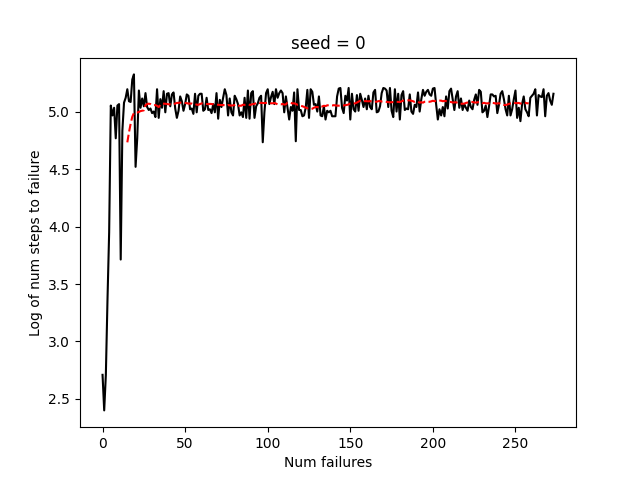
\includegraphics[width=0.5\linewidth]{src/output/control_0.png}
      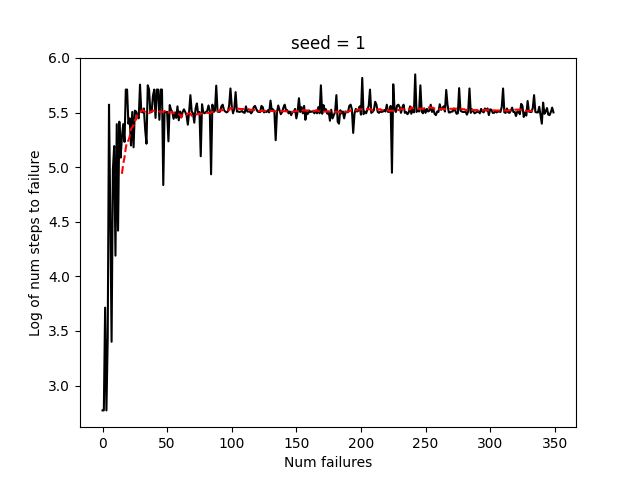
\includegraphics[width=0.5\linewidth]{src/output/control_1.png}
      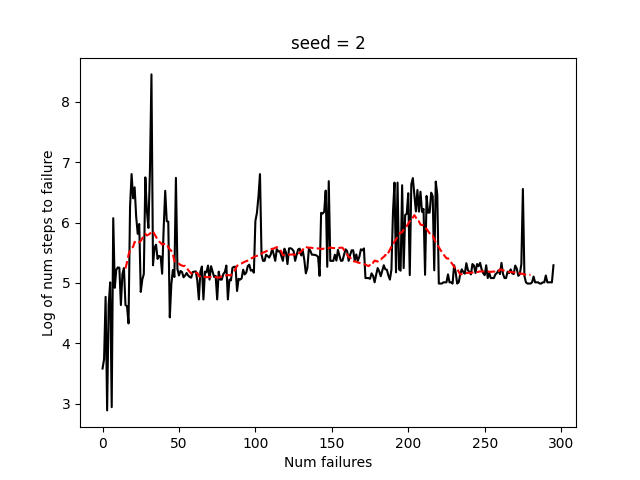
\includegraphics[width=0.5\linewidth]{src/output/control_2.png}
      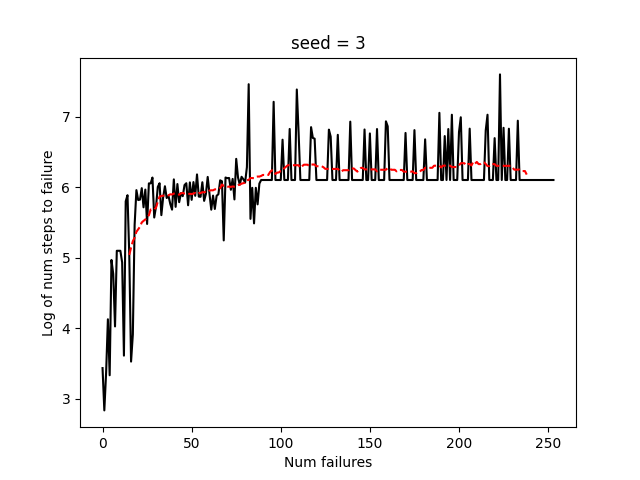
\includegraphics[width=0.5\linewidth]{src/output/control_3.png}
      \caption{Learning curve of algorithm for 4 different random seed.}
      \label{learning-curve}
    \end{figure}
  \end{enumerate}
\end{solution}

\end{document}